\section{Claims that did not survive}\label{sec:audit}

A ratchet is worth only as much as its pawl. Several recorded results were
corrected once the reference was matched, native work was priced, or the
evidence was replayed. Each correction is recorded in the source with a
dated note; frozen evidence is never rewritten. Figure~\ref{fig:audit}
shows the before and after values. Every correction moved IC's position
against rho \emph{down}, and several moved it from apparently ahead of rho
to behind it.

\begin{figure}[t]
\centering
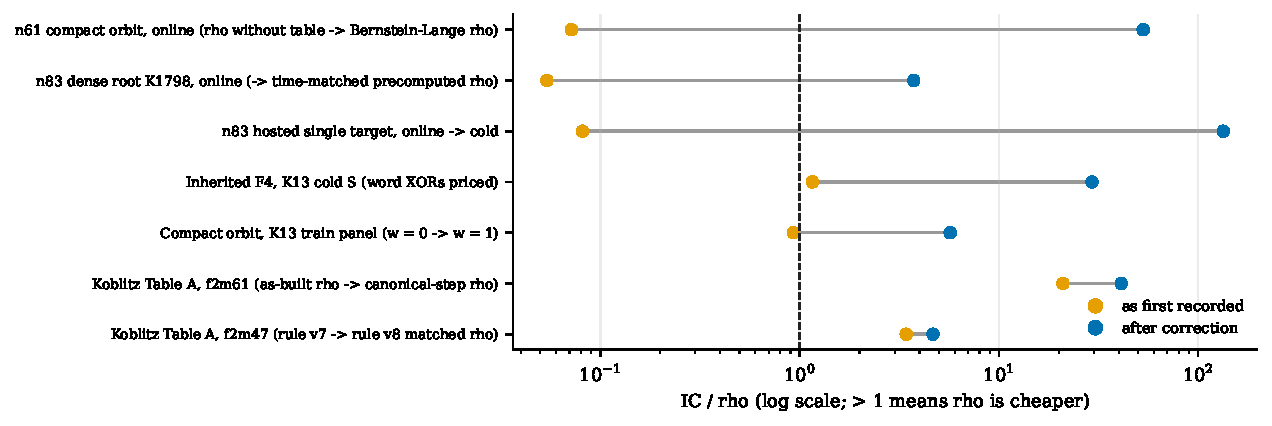
\includegraphics[width=\linewidth]{figures/fig-audit.pdf}
\caption[]{IC/rho as first recorded (orange) and after correction (blue), on
the boundary the correction used. Values left of the dashed line had
claimed IC ahead of rho. Sources: \art{figures/data.json}.}
\label{fig:audit}
\end{figure}

\paragraph{1. Every online win is retired.} The one-target online ladder
compared IC \emph{with} a retained table against rho \emph{without} one:
\begin{itemize}
\item $13.94\times$ $[9.81,19.13]$ over strong rho at $n=61$, on 64 targets;
\item $18.53\times$ at $n=83$ with a dense root index;
\item $7.29\times$ and $12.29\times$ on hosted single targets at $n=71$
  and $n=83$.
\end{itemize}
Given a distinguished-point table no larger than IC's pair table,
Bernstein--Lange preprocessing rho~\cite{bl2012} is $53$--$317\times$ faster
online at $n=41,53,61$ on the same 64 targets (benchmarks row
\texttt{20261014-ic-next10-09-equal-advice}). At $n=83$, rho with a table
matched to IC's set-up time or memory wins every pair: $3.74\times$
time-matched and $40.61\times$ memory-matched against K3300, and
$81.5$--$395.5\times$ against K600 (benchmarks row
\texttt{20261016-n83-precomputed-rho-control}). Cold, the hosted $n=83$
point is $133.7\times$ rho. Those online rows measured what a table buys,
and generic rho buys more per byte. The within-IC result survives: K1798's
probe reduction over K1500 at $n=83$ (from $300{,}021.9$ to $169{,}069.8$
probes per relation).

\paragraph{2. Pricing native work moved two arms.}
\begin{itemize}
\item \emph{Inherited F4 at $n=13$.} Its $S=16.7$, close to rho's $14.4$,
  left its Boolean word XORs unpriced. Priced, $S=421.4$
  (\art{research/ecbench_rootfind_faster_20261014/}).
\item \emph{F4 pricing change.} The pricing change (\#1774, $0.002304$ GAE
  per word XOR) made every earlier F4 $S$ a lower bound. A separate
  algorithmic change (\#1862) raised counted work
  (\art{research/f4_pricing_jump_20261018/README.md}).
\item \emph{Compact orbit at $n=13$.} Earlier quoted at $1.08\times$ rho as a
  lower bound, it reads $0.93$, $1.53$ and $5.7\times$ the strong rho at
  $w=0,0.1,1$, so the pair is unresolved inside the band
  (\art{research/ic_frontier_campaign_20261015/select/SELECTION.md}).
\end{itemize}

\paragraph{3. Matching the rho reference.}
\begin{itemize}
\item \emph{Rule v8.} Matching the rho reference raised the Koblitz gap by
  $1.30$--$1.58\times$ at every size (\S\ref{sec:distance}).
\item \emph{The standing rho improved.} Ecbench's standing
  \texttt{rho.signed\_frobenius\_strong} now runs at $0.802\times$ its
  former instruction count with identical GAE, and the strong Koblitz rho
  executes 718 instructions per step instead of 1{,}196. Counted-unit
  comparisons are unaffected. Wall-time comparisons against the older rho
  overstate IC by up to that factor.
\item \emph{Two rho studies on the prime side.} Choosing the better of
  $P\pm R$ cuts steps by $1.129\times$. Signed $\sigma$ steps on
  ECC2K-130 cut GPU time to $0.961$--$0.970$. Neither is yet in a campaign
  arm.
\end{itemize}

\paragraph{4. A replay regression, and its root cause.} The root-finder
ecbench session was recorded with a replay certificate of 120 of 168
identical records; the 48 mismatches were all in inherited F4's word-XOR
counts. On current \texttt{main} it replayed only 72 of 168, with
mismatches in all four IC arms. The validation sweep of 19--20 October
isolated the cause (\art{research/validation_sweep_20261019/D-known-issues/item1_cross_isa_20261020/RESULT.md}):
\begin{itemize}
\item \emph{Cause.} The x86-only BMI2 word-wise rewrite in
  \art{src/cryptanalysis/inherited_f4.rs} charges a different word-XOR
  count from the portable path, for example $301{,}961$ against
  $300{,}531$. The method identity does not record which path ran.
\item \emph{Confirmation.} With that branch disabled, x86 reproduces all
  168 of 168 records. An aarch64 build under emulation also reproduces 168
  of 168. An independent rerun repeated the result.
\item \emph{What it rules out.} Compiler version, source drift since the
  archive, and the two later pricing changes.
\end{itemize}
Scalars, trial counts and charged GAE outside F4 are unaffected. F4 $S$ is
not comparable across instruction-set architectures unless the path is
stated. Until the method identity records the path, the root-finder rows
rest on the original receipt.

\paragraph{5. Reported cells that compared unlike statistics.} The
u64-rootbatch rank and per-target cells compared a fastest run with a
median, and were corrected from $2.95\times$ and $6.09\times$ to $2.47\times$
and $5.00\times$ (\S\ref{sec:setup}). The $n=83$ stacked producer's
``$360\to94.4$'' cold-gap history mixed a ratio from another run; paired
within the run it is $305.8\to94.4$ (\S\ref{sec:setup}).

\paragraph{6. Results resting on faulty code or wrong references.}
\begin{itemize}
\item \emph{Plane-quartic IC.} Its $S$ values of $650{,}896$ to
  $3.79\cdot10^7$ rest on a degree-3 reduction in
  \art{research/ghs_cubic_quartic_ic_20261012/quartic_ic.rs} that merges
  distinct classes (reported in an open pull request). Recoveries are still
  checked against the planted scalar, but relation counts and $S$ are
  unverified.
\item \emph{Volcano census crater.} A claim that IC is 22--25\% cheaper on
  the volcano crater was withdrawn, because the crater's rho reference
  should have been the cubic-automorphism rho. Against it, IC is
  $84.9\times$ rho at $w=0$
  (\art{research/volcano_ecdlp_census_20261017/REPORT.md}, erratum A3).
\end{itemize}

\paragraph{Reading.} None of these corrections removes an IC improvement
against its own incumbent. They correct the \emph{distance to rho}, which
is the quantity most exposed to an unmatched reference or an unpriced
counter. This is why the gate of \S\ref{sec:gate} asks for a matched,
band-priced rho on every row.
